\documentclass{article}
\usepackage[utf8]{inputenc}
\usepackage[T1]{fontenc}
\usepackage[utf8]{inputenc}
\usepackage{graphicx}
\usepackage[a4paper, total={6.5in, 8.5in}]{geometry}
\setcounter{secnumdepth}{4}
\usepackage{hyperref}
\usepackage{color}
\usepackage{booktabs}
\usepackage{tabularx}
\usepackage{amsmath}
\usepackage{textcomp}
\usepackage{xcolor}
\usepackage{listings}
\usepackage{enumitem}
\usepackage{minted}
\usepackage{tikz}
\usepackage{ccicons}
\usepackage{fancyhdr}
\usepackage{pgfplots}
\usepackage[
type={CC},
modifier={by-nc-sa},
version={4.0},
]{doclicense}
\pgfplotsset{compat=newest}
\usetikzlibrary{arrows.meta, positioning}

\definecolor{highlight}{rgb}{0.22,0.45,0.70}

\title{Classification of wireless transmitters}
\author{Alessandro Amella, Marian Abuziloaie}
\date{\today}

\makeindex

\pagestyle{fancy}
\fancyhf{} % Clear header and footer
% \fancyhead[C]{\nouppercase{\leftmark}} % Current section at the top
\fancyfoot[C]{\thepage} % Page numbers at the bottom
\renewcommand{\headrulewidth}{0.4pt} % Header rule
\renewcommand{\footrulewidth}{0pt} % Footer rule

\begin{document}

\maketitle

% \doclicenseThis%

% \tableofcontents

% \clearpage

\section{Introduction}
The aim of this project is to determine the number of wireless transmitters based on observed hardware imperfections. This involves analyzing a dataset of 19,200 samples, each described by eight features that represent various radio frequency impairments. This report outlines our approach to preprocessing the data, selecting and training a model, and discussing the results obtained.

\section{Problem Description}
Wireless transmitters often exhibit hardware imperfections that can impact their performance. The dataset provided includes measurements of eight such imperfections, including Carrier Frequency Offset (CFO), gain imbalance, and Error Vector Magnitude (EVM). Our task is to use this data to try and estimate the number of transmitters.

\section{Methodology}

\subsection{Data Examination and Preprocessing}
Upon loading the dataset, preliminary examination revealed that it consists of floating-point and integer values, with a few columns not directly related to the classification task, such as the first (representing the trasmitter number in the dataset), \texttt{time [s]} and \texttt{cfo\_meas}. These were removed to focus on the eight features of interest. The data was then standardized using Scikit-learn's StandardScaler to ensure all features contribute equally to the analysis.

\subsection{Model Selection}
Given the nature of the task — classifying transmitters based on their hardware imperfections — we opted for a KMeans clustering approach. This decision was supported by inspection of the silhouette scores for varying numbers of clusters, suggesting that six clusters provide a good balance between within-cluster similarity and between-cluster difference.

\subsection{Model Training}
With the number of clusters determined, we trained a KMeans model on the standardized data. The process involved initializing the model with six clusters and a random state for reproducibility, then fitting it to the data to perform the classification.

\section{Results}
Upon training the model, we classified the transmitters into six distinct groups based on their impairment characteristics. The mean values of the features for each cluster, as presented in the following table, reveal notable differences in hardware imperfections across clusters.

\begin{table}
\centering
\label{tab:cluster_stats}
\begin{tabular}{lrrrrrrrr}
\toprule
Cluster & cfo\_demod & gain\_imb & iq\_imb & or\_off & quadr\_err & ph\_err & mag\_err & evm \\
\midrule
0 & -471.55 & 0.056 & -31.99 & -30.71 & 2.86 & 1.30 & 2.13 & 3.09 \\
1 & -371.65 & -0.015 & -30.06 & -36.06 & -3.60 & 1.25 & 2.67 & 3.41 \\
2 & -393.08 & 0.067 & -45.82 & -27.53 & 0.37 & 1.07 & 0.53 & 1.91 \\
3 & 448.01 & 0.069 & -34.81 & -28.60 & 2.04 & 1.09 & 1.54 & 2.43 \\
4 & -707.82 & 0.081 & -38.32 & -28.85 & 1.30 & 1.15 & 1.07 & 2.25 \\
5 & -376.06 & -0.039 & -29.61 & -37.73 & -3.76 & 1.57 & 3.52 & 4.31 \\
\bottomrule
\end{tabular}
\caption{Mean values of features by cluster.}
\end{table}



Figure 1 shows the silhouette score analysis used to determine the optimal number of clusters.

% Placeholder for figure; replace with your code's plot if applicable.
\begin{figure}[ht]
\centering
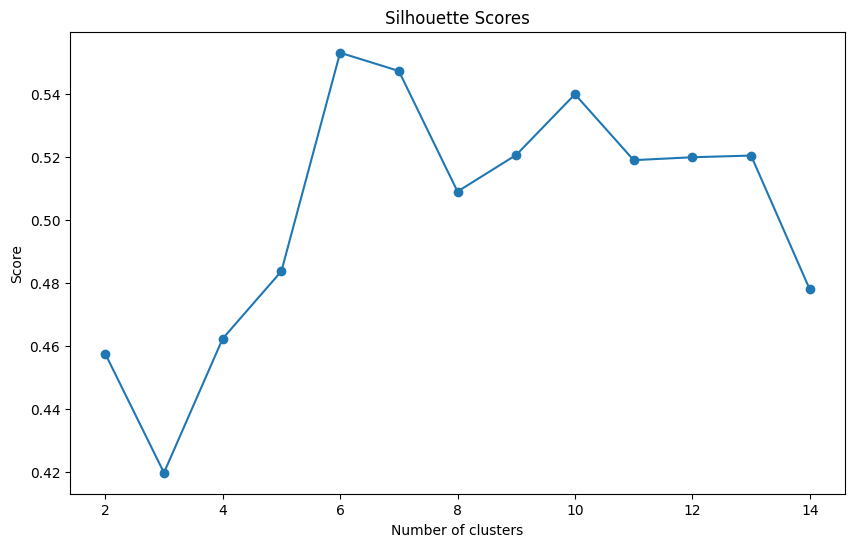
\includegraphics[width=0.8\textwidth]{silhouette.png}
\caption{Silhouette score analysis for determining the number of clusters.}
\label{fig:silhouette}
\end{figure}

\section{Conclusions}
This project demonstrates the utility of machine learning techniques in classifying wireless transmitters based on their hardware imperfections. The KMeans clustering model, chosen for its simplicity and effectiveness, successfully grouped transmitters into clusters based on the magnitude of their impairments. After fine-tuning several parameters, we determined that the most probable number of clusters is 6.


\appendix

\vspace*{\fill}

% \vspace{2em}
\hrulefill
\vspace{1em}

\textbf{Alessandro Amella, Marian Abuziloaie \textcopyright{} 2024}

\end{document}